% !TEX root = mainthesis.tex

%Chapter 3


\renewcommand{\thechapter}{3}

\chapter{Manipulation and detection of ultra-cold atoms}
\label{ch:Ch3}

All of the experiments described in this thesis were performed using ultracold clouds of $\Rb87$. In this Chapter I describe the techniques and interactions that make our experiments possible. This Chapter is not an extensive survey of atomic physics but rather covers the topics that are most relevant to my experiments. The references I included are helpful if the reader is interested in learning the details of the derivations or wants to expand on a given topic. I start by describing the electronic structure of $\Rb87$ in Section~\ref{sec:electronic_structure}. In Sections~\ref{sec:zeeman_effect} and~\ref{sec:atom-lignt_interactio n} I describe atomic interactions with external fields that are necessary for the creation, manipulation and detection of ultracold atoms. First I review the interactions of atoms with magnetic fields and its application to magnetic trapping. Then I describe the foundations of atom-light interactions that make possible both laser cooling and trapping of atoms and give rise to Raman induced transitions. In Section~\ref{sec:absorption imaging} I discuss resonant absorption imaging which is used to detect atoms after all our experiments are performed. Finally in Section~\ref{sec:quantum_coherent_dynamics} I discuss coherent processes that use the magnetic and electric dipole interaction and are relevant to the experiments presented in Chapters~\ref{ch:Fourier_spectroscopy}, \ref{ch:clock_states} and \ref{ch:Rashba}. 

%Both the cooling and trapping of atoms as well as the engineering of interesting potentials and detection of atoms rely on the interaction of atoms with electromagnetic fields as well as with static and oscillating magnetic fields. 
\section{Electronic structure of $^{87}$Rb}
\label{sec:electronic_structure}

\begin{figure*}[htb]
\begin{center}
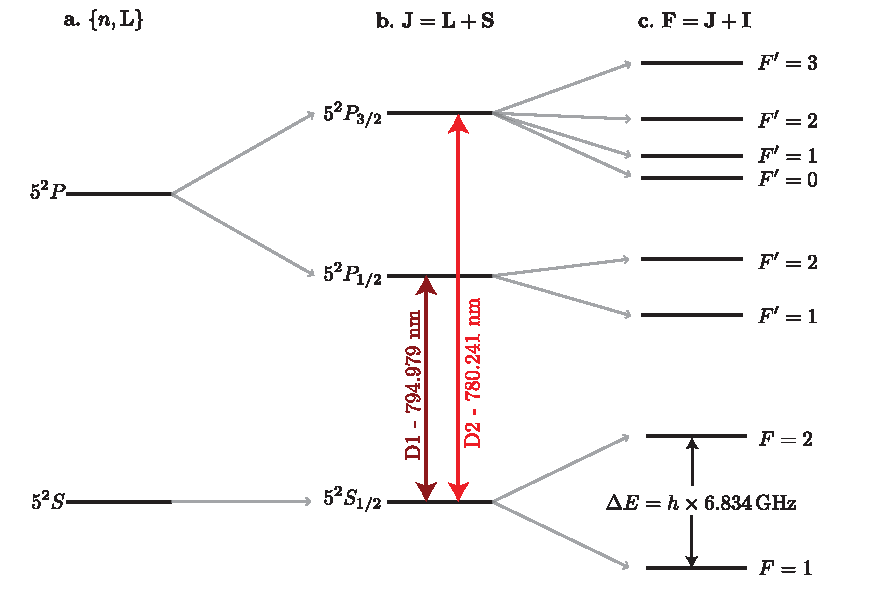
\includegraphics[]{Figures/Chapter3/Rb_structure.pdf}
\caption[$\Rb87$ level structure]{$\Rb87$ level structure (not to scale). {\bf a.} Ground and first excited state electronic configuration of $\Rb87$ given by the $\{n,\mathbf{L}\}$ quantum numbers. {\bf b.} The interaction between the orbital angular momentum and the spin of the electron leads to the fine structure splitting of orbitals with $L>0$. The splitting of the $5^2P$ line gives rise to the D1 and D2 lines. {\bf c.} The interaction between the total angular momentum and the nuclear spin causes the fine structure levels to split further into states characterized by the quantum number $F$.}
\label{fig:Rb_structure}
\end{center}
\end{figure*}

Rubidium (Rb) is an Alkali metal (also Li, which exists in our vacuum chamber but was never used). Alkali metals correspond to the first group (leftmost column) of the periodic table and are characterized by having a single valence electron, which makes the description of their internal structure much simpler than that of other elements. We can describe the state of an electron in an atom by its angular momentum $\mathbf{\hat{L}}$ and its spin $\mathbf{\hat S}$. Because of Pauli's exclusion principle there can not be two electrons with the same quantum numbers and in multi-electron atoms they tend to fill `shells' of different angular momentum values, historically labeled by the letters $S,\ P,\ D,\ F,\ ...$\footnote{These terms were used to describe the lines in the emission spectra when they were first discovered. $S$ stands for sharp, $P$ for principal $D$ for diffuse and $F$ for further noted} (corresponding to $L=0,\ 1,\ 2,\ 3,\  ...$). In particular, Rb has 4 filled shells and one electron in the $5S$ shell, where the number $5$ corresponds to the principal quantum number $n$. Figure~\ref{fig:Rb_structure} shows the energy levels of the ground state $5S$ and its closest $5P$ orbital. %In the absence of interactions, the $m_l$ sublevels within an orbital are degenerate.

The atomic level structure is modified by relativistic effects. The relativistic treatment of the electron's motion gives rise to an interaction between the electron's intrinsic magnetic moment (the spin) $\mathbf{\hat S}$ and the orbital angular momentum $\mathbf{\hat L}$. This spin-orbit coupling interaction $\hat H_{\rm {fs}} = A_{\rm{fs}} \mathbf{L}\cdot\mathbf{S}$ causes the fine structure splitting of the electronic orbitals into levels with different total electronic angular momentum $\mathbf{\hat J}=\mathbf{\hat L}\cdot\mathbf{\hat S}$. Figure~\ref{fig:Rb_structure}b show the $5^2S_{1/2}$, $5^2P_{1/2}$ and $5^2P{3/2}$ electronic configurations that arise from this splitting, where I introduced the spectroscopic notation $n^{2S+1}L_{J}$ that indicates the values of the relevant quantum numbers. For $S$ ($L=0$) orbitals $J=1/2$ is the only possible value and the levels are not split. For the $P$ orbital ($L=1$) $J$ and a single electron with $S=1/2$, $J$ can be $1/2$ or $3/2$ and the $P$ orbital splits into two levels. The $5^2S_{1/2}\rightarrow 5^2P_{1/2}$ is known as the D1 line and has wavelength $\lambda=\unit[794.979]{nm}$ and $5S_{1/2}\rightarrow 5P_{3/2}$ transition is known as the D2 line and has $\lambda=\unit[790.241]{nm}$ \cite{Steck}. 

The atomic level structure gets further modified by the magnetic interaction of the electron with the nuclear spin $\mathbf{I}$. This is another kind of spin-orbit interaction that gives rise to the hyperfine splitting of the atomic levels which can be described by the Hamiltonian $\hat H_{\rm{hfs}} = A_{\rm{hfs}}\mathbf{I}\cdot\mathbf{J}$. A complete derivation of $\hat H_{\rm{hfs}}$ can be found in~\cite{schwartz_theory_1955}. The hyperfine levels correspond to different values of the total angular momentum $\mathbf{\hat F}=\mathbf{\hat J}+\mathbf{\hat I}$. For $\Rb87$ $I=3/2$~\cite{Steck} which results in the level structure shown in Figure~\ref{fig:Rb_structure}c. 



\section{Interaction between atoms and magnetic fields}
\label{sec:zeeman_effect}

Atoms have an intrinsic magnetic moment that is given by the sum of nuclear and electronic moments
%
\begin{equation}
	\boldsymbol{\hat \mu}=-\frac{\mu_B}{\hbar}(g_S\mathbf{\hat{S}}+g_L\mathbf{\hat L}+g_I\mathbf{\hat I})%=\frac{\mu_B g_F}{\hbar} \mathbf{\hat F}
\end{equation}
%
where $\mu_B$ is the Bohr magneton and $g_S$, $g_L$ and $g_I$ are the `$g$-factors' corresponding to the spin, orbital and nuclear angular momentum. In the presence of an external magnetic field $\mathbf B$, the internal levels of an atom get modified due to the Zeeman~\cite{Zeeman_effect} interaction
%
\begin{equation}
	\hat{H}_{\rm{Zeeman}}=-\boldsymbol{\hat \mu}\cdot\mathbf{B}.
	\label{eq:zeeman_hamiltonian}
\end{equation}
%
If the energy shift due to the Zeeman interaction is small compared to the hyperfine splitting so that $F$ is a good quantum number we can write
\begin{equation}
	\hat{H}_{\rm{Zeeman}}=\frac{\mu_B g_F}{\hbar}\mathbf{\hat F}\cdot\mathbf{B}
\end{equation}
%
where is the hyperfine Land\'e $g$-factor
%
\begin{equation}
	g_F=g_J\frac{F(F+1)-I(I+1)+J(J+1)}{2F(F+1)}+g_I\frac{F(F+1)+I(I+1)-J(J+1)}{2F(F+1)}
\end{equation}
and
%
\begin{equation}
	g_J\approx=1+\frac{J(J+1)+S(S+1)-L(L+1)}{2J(J+1)}.
\end{equation}
%
is the Land\'e $g$-factor associated to the total electronic angular momentum $J$. The total energy shifts can be calculated by diagonalizing the full atomic Hamiltonian including the fine and hyperfine structure terms. Figure~\ref{fig:Zeeman_splitting} shows the energies of the $m_F$ levels in the $F=1$ and $F=2$ manifolds of the $5^2S_{1/2}$ electronic ground state of $\Rb87$ as a function of magnetic field. If the magnetic field is small then the Zeeman term can be treated as a perturbation to the atomic Hamiltonian and the energy split is linear with the magnitude of the field $E_{m_F}=g_F\mu_B m_FB$, what is known as the `linear Zeeman regime' where $F$ and $m_F$ are good quantum numbers. In contrast, in the `Pachen-Back regime' at large magnetic fields\footnote{A couple orders of magnitude larger than the fields we operate at.} the Zeeman term dominates over the fine and hyperfine terms and therefore the good quantum numbers of the system are $J$ and $m_J$. Our experiments typically operate in an intermediate regime ($B\sim 10-30\,\rm{G}$, the gray box in Figureº~\ref{fig:Zeeman_splitting}) where the energy of $m_F=0$ gets a small shift in energy that is quadratic in $B$. For atoms in $F=1$ we define this quadratic Zeeman shift as $\epsilon=E_0-(E_{+1}-E_{-1})/2$, where $E_{m_F}$ is the Zeeman shift for state $m_F$.

\begin{figure*}[htb]
\begin{center}
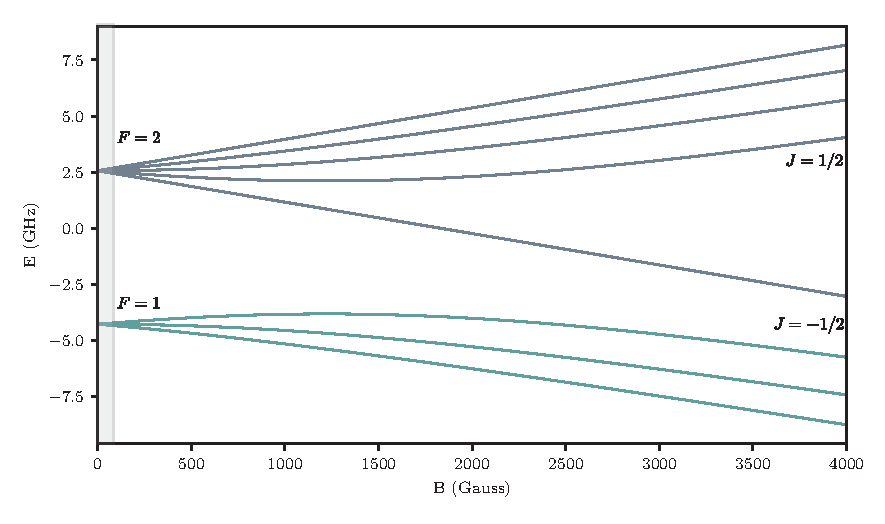
\includegraphics[]{Figures/Chapter3/anotated_zeeman_spltting.pdf}
\caption[Zeeman splitting of the $5^2S_{1/2}$ manifold of $\Rb87$]{Zeeman splitting of the $5^2S_{1/2}$ manifold of $\Rb87$. At small magneric fields $F$ and $m_F$ are good quantum numbers describing the system and at large magnetic fields (Pachen-Back regime) the states are described by the $J$ and $m_J$. Our experiments operate in the regime marked by the small gray box ($B<\unit[35]{G}$).}
\label{fig:Zeeman_splitting}
\end{center}
\end{figure*}

For the particular case of $J=1/2$ (like the ground state of Alkalis) the Zeeman energies can be found analytically using the Breit-Rabi formula~\cite{breit_measurement_1931}
%
\begin{equation}
	E_{m_F}=-\frac{1}{2(2I+1)}+\frac{\mu_Bg_Im_FB}{\Delta E_{\rm{hf}}}+\frac{1}{2}\sqrt{1+\frac{4m_F}{2I+1}x+x^2},
	\label{eq:Breit_rabi}
\end{equation}
%
where $\Delta E_{\rm{hf}}=A_{\rm{hf}}(J+1/2)$ and $x=(g_J-g_I)\mu_B B_z/\Delta E_{\rm{hf}}$. Figure~\ref{fig:Zeeman_splitting} shows the energies of the $m_F$ levels for the $F=1$ and $F=2$ manifolds of $\Rb87$.

\subsection{Magnetic trapping}
\label{sec:magnetic_trapping}
The sign of the Zeeman energy for different $m_F$ states can be used to create state-dependent traps for atoms. In the lab, we implement magnetic traps using quadrupole magnetic fields produced by a pair of anti-Helmholtz coils. The magnetic field near the center of the coils can be written as
%
\begin{equation}
	\mathbf{B}=B'(x\ex+y\ey-2z\ez) + \mathbf{B}_0
\end{equation}
%
where $\mathbf{B}_0$ is a constant magnetic field, for simplicity I will assume that $\mathbf{B}_0=B_0\ez $. The Zeeman Hamiltonian gives a trapping potential
%
\begin{align}
	U(\mathbf{r})&=g_F\mu_B m_F B \nonumber \\
	&=g_F\mu_B m_F B'\sqrt{x^2+y^2+4\left(z-\frac{B_0}{2B'}\right)^2} \nonumber \\
	& \approx g_F\mu_B m_F B'\left(\rho+2\left\vert z-\frac{B_0}{2B'}\right\vert\right)
	\label{eq:quadrupole_trap}
\end{align}
%
where $\rho^2=x^2+y^2$ and the approximation on the second line is valid for small displacements from the trap center. 

The sign of the magnetic moment determines which states can be trapped. For $\Rb87$ the $\ket{F=1, m_F=-1}$, $\ket{F=2, m_F=2,1}$ are magnetically trappable. The state $\ket{F=2, m_F=0}$ is also weakly magnetically trappable due to the quadratic Zeeman shift. 

In addition to generating trapping potentials, we use quadrupole fields before imaging the atoms to generate state-dependent forces that separate the different $m_F$ states in a similar way as the Stern-Gerlach (SG) effect.

\section{Interaction between atoms and electric fields}
\label{sec:atom-lignt_interactio n}

In this section, I will discuss the interaction between atoms and electric fields. After laying the foundations I will discuss applications using off-resonant electromagnetic radiation such as optical dipole traps and Raman transitions. I will not cover laser cooling which has been covered extensively in the literature~\cite{metcalf_deceleration_1999,phillips_nobel_1998} and PhD theses from previous group members~\cite{CampbellThesis,PriceThesis}. 

In the presence of an electric field $\mathbf E$, an atom can become polarized and therefore its energy levels get modified by the Stark effect~\cite{stark_beobachtungen_1914}. If the electric field is spatially uniform with respect to the atom's size we consider the electric field as a classical object and its effect on the atom can be described by the Hamiltonian~\cite{Cohen-Tanoudji}  
%
\begin{equation}
\hat{H}_{\rm{dip}} = -\mathbf{\hat d}\cdot\mathbf{E},
\label{eq:dipole_ham}	
\end{equation}
%
where $\mathbf{\hat d}=-e\sum_j r_j$ is the atomic dipole operator, $e$ is the electron charge and $\hat r_j$ are the position operators of the atom's electrons relative to the center of mass of the atom. This approximation, known as the dipole approximation, is valid for electromagnetic radiation when the wavelength is much larger than the size of an atom $\lambda\gg r_{\rm{atom}}$~\cite{SteckTextbook}. 

First I consider the simplified case a two-level system interacting with a coherent electromagnetic field $\mathbf{E}=\mathbf{E}^{(+)}e^{-i\omega t}+\mathbf{E}^{(-)}e^{i\omega t}$, where $\mathbf{E}^{(\pm)}=\hat{\epsilon}E^{(\pm)}$ are the positive/negative frequency components of the field, $\hat{\epsilon}$ the polarization, and $\omega$ is the angular frequency. It can be shown sing second-order perturbation theory that Stark shift of the ground state is
%
\begin{align}
 	\Delta E_g&=-\frac{2\omega_{eg}\vert\bra{g}\hat{\epsilon}\cdot\mathbf{d}\ket{e}\vert^2\vert E^{(+)}\vert^2}{\hbar(\omega_{eg}^2-\omega^2)}\nonumber \\
 	&= -\frac{1}{2}\alpha(\omega) E^2
 \end{align} 
%
where $\omega_{eg}=(E_e-E_g)/\hbar$ is the angular frequency associated to the energy splitting of the two states and  $\alpha(\omega)$ is a dynamic polarizability. Things are a bit more complicated with real atoms though, and we need to take into account all the atomic levels. Furthermore, there are degeneracies associated to the different angular momentum states so we have to be more careful with the orientation of the atom and the field. To take these effects into account one can introduce a generalization of the polarizability~\cite{SteckTextbook,deutsch_quantum_2010} which takes the form
%
\begin{align}
	\alpha_{\mu\nu}(\omega)&=\sum_j\frac{2\omega_{jg}\bra{g}d_\mu\ket{e_j}\bra{e_j}d_\nu\ket{g_j}}{\hbar(\omega_{jg}^2-\omega^2)}\nonumber \\
	&= \sum_{F',\ m_{F'}}\frac{2\omega_{F'F}\bra{F,m_F}d_\mu\ket{F', m_{F'}}\bra{F', m_{F'}}d_\nu\ket{F,m_F}}{\hbar(\omega_{F'F}^2-\omega^2)}.
\end{align}
%
Here  $\ket{e_j}$ represent the excited states and $\omega_{jg}=(E_j-E_g)/\hbar$ and the expression in the second line corresponds the polarizability for the hyperfine levels of an atom in the ground state $\ket{F, m_F}$. We can therefore write an effective Hamiltonian for the Stark shift as 
%
\begin{align}
	\hat{H}_{\rm{Stark}}&=-\alpha_{\mu\nu}(\omega)E_{\mu}^{(+)}E_{\nu}^{(-)}.
\end{align}
%

The polarizability is a rank-2 tensor operator and can be represented by 3 irreducible tensor operators (see~\cite{SteckTextbook} for a complete derivation). In the limit of small magnetic fields so that $F$ and $m_F$ are good quantum numbers describing the state of the atom $\ket{n, F, m_F}$ the dipole Hamiltonian in this representation takes a convenient form
%
\begin{align}
	\hat{H}_{\rm{Stark}}= &\alpha^{(0)}(\mathbf{E}^{(-)}\cdot\mathbf{E}^{(+)}) 
	+i\alpha^{(1)}(\mathbf{E}^{(-)}\times\mathbf{E}^{(+)})\cdot\mathbf{\hat{F}}  \nonumber \\ 
	&+ \alpha^{(2)}E_i^{(-)}E_j^{(+)}	\left(\frac{1}{2}(F_iF_j+F_jF_i)-\frac{1}{3}\mathbf{\hat F}^2\delta_{i,j}\right)\Big],
	\label{eq:light_matter_coupling}
\end{align}

% where $\mathbf{E}^{(\pm)}$ are the possitive/negative frequency components of the field. $\alpha_{\mu\nu}(\omega)$ can be found by looking at the (time averaged) shift in the energy of a given state state using second order time-dependent perturbation theory~\cite{SteckTextbook,deutsch_quantum_2010}. For the ground state $\ket{g}$ the polarizability takes the form 
% %
% \begin{equation}
% 	\alpha_{\mu\nu}(\omega)=\sum_j\frac{2\omega_{jg}\bra{g}d_\mu\ket{e_j}\bra{e_j}d_\nu\ket{e_j}}{\hbar(\omega_{jg}^2-\omega^2)},
% \end{equation}
% %
% where $\ket{e_j}$ represent the excited states and $\omega_{jg}=(E_j-E_g)/\hbar$. The dipole operator is a rank-2 tensor and can be represented by 3 irreducible tensor operators (see~\cite{SteckTextbook} for a complete derivation). In the limit of small magnetic fields so that $F$ and $m_F$ are good quantum numbers describing the state of the atom $\ket{n, F, m_F}$ the dipole Hamiltonian in this representation takes a convenient form
%
% \begin{align}
% 	\hat{H}_{\rm{dip}}= &\alpha^{(0)}(\mathbf{E}^{(-)}\cdot\mathbf{E}^{(+)}) 
% 	+i\alpha^{(1)}(\mathbf{E}^{(-)}\times\mathbf{E}^{(+)})\cdot\mathbf{\hat{F}}  \nonumber \\ 
% 	&+ \alpha^{(2)}E_i^{(-)}E_j^{(+)}	\left(\frac{1}{2}(F_iF_j+F_jF_i)-\frac{1}{3}\mathbf{\hat F}^2\delta_{i,j}\right)\Big],
% 	\label{eq:light_matter_coupling}
% \end{align}
%
where $\alpha^{(0)}$, $\alpha^{(1)}$ and $\alpha^{(2)}$ are the scalar, vector and tensor polarizabilities respectively and $\hat{\mathbf{F}}$ is the total angular momentum operator. For all our experiments $\alpha^{(2)}$ is very small so I will limit the discussion to the effect of the first two terms. The scalar term is responsible for the dipole force that allow us to trap atoms using off-resonant light and the vector component is necessary for engineering spin-orbit coupling and other spin-dependent potentials through two-photon processes. 

\subsection{Scalar polarizability}
\label{sec:scalar_light_shift}

The scalar polarizability takes the form
%
\begin{equation}
	\alpha^{(0)}=\sum_j\frac{2\omega_{jg}\vert\bra{g}\mathbf{d}\cdot\hat{\epsilon}\ket{e_j}\vert^2}{\hbar(\omega_{jg}^2-\omega^2)},
\end{equation}
%
where the matrix element can be expressed in terms of the Clebsch-Gordan coefficients and the reduced matrix element using the Wigner-Eckart theorem~\cite{Sakurai}. For the ground state of an Alkali atom ($J=1/2$) and if the detuning is large compared to the hyperfine splitting the expression above gets simplified to
%
\begin{equation}
	\alpha^{(0)}\approx\sum_{J'}\frac{2\omega_{JJ'}\vert\langle J=1/2 \| \mathbf{d}\|J'\rangle\vert^2}{3\hbar(\omega_{JJ'}^2-\omega^2)}.
\end{equation}
Due to the second order-perturbation theory treatment, the scalar polarizability can be interpreted as arising from a two-photon process where the atom absorbs an off-resonant (virtual) photon and then returns to its initial state by emitting a photon. 

The dipole matrix elements needed to compute the polarizability are related to the transition scattering rate via Fermi's golden rule~\cite{Sakurai,SteckTextbook}
\begin{equation}
	\Gamma_{JJ'}=\frac{\omega_{JJ'}^2}{3\pi\epsilon_0\hbar c^3}\frac{2J+1}{2J'+1}\vert\langle J \| \mathbf{d}\|J'\rangle\vert^2,
\end{equation}
%
and combining this with the expression for the intensity of the electric field $I(\r)=2\epsilon_0c\vert \mathbf{E}(\r)\vert^2$ it can be shown that for linearly polarized light the energy of the ground state manifold is shifted by
\begin{equation}
	U(\omega,\r)=-\frac{\pi c^2 I(\r)}{2}\left[ \frac{\Gamma_{\rm{D1}}}{\omega_{\rm{D1}}^3}\left(\frac{1}{\omega+\omega_{\rm{D1}}}-\frac{1}{\omega-\omega_{\rm{D1}}}\right)+\frac{2\Gamma_{\rm{D2}}}{\omega_{\rm{D2}}^3}\left(\frac{1}{\omega+\omega_{\rm{D2}}}-\frac{1}{\omega-\omega_{\rm{D2}}}\right)\right],
\end{equation}
%
where only the the most significant contribution from the closest transitions  (the D1 and D2 lines) are included. Here $U(\r)$ is related to the real part of the polarizability which is in fact a complex valued number. So far I have only considered a real valued polarizability by assuming the excited states have an infinitely long lifetime. However, in reality the atom can spontaneously emit photons and decay. This exponential decay can be accounted for by adding an imaginary contribution to the energies $\omega_D\rightarrow\omega_D+i\Gamma_D\omega^3/\omega_D^3$ of the D1 and D2 transitions~\cite{grimm_optical_2000}. The scattering rate is related to the imaginary part of the polarizability and is given by
%
\begin{equation}
	\Gamma(\omega,\r)=\frac{\pi c^2I(\r)}{2\hbar}\left[ \frac{\Gamma_{\rm{D1}}\omega^3}{\omega_{\rm{D1}}^6}\left(\frac{1}{\omega+\omega_{\rm{D1}}}-\frac{1}{\omega-\omega_{\rm{D1}}}\right)^2+\frac{2\Gamma_{\rm{D2}}\omega^3}{\omega_{\rm{D2}}^6}\left(\frac{1}{\omega+\omega_{\rm{D2}}}-\frac{1}{\omega-\omega_{\rm{D2}}}\right)^2\right]
	\label{eq:scattering}
\end{equation}

The energy shift $U(\omega,\r)$ is a conservative term and is related to dipole trapping, while the scattering term $\Gamma(\omega,\r)$ is dissipative and is important for laser cooling. In the context of engineering potentials for ultracold atoms with off-resonant light, the scattering is translated into heating because every time an atom emits a photon with angular frequency $\omega_L$ it gets a recoil momentum $\hbar\k_L$. If the frequency $\omega$ satisfies the relation $\omega+\omega_{\rm D}\gg\omega-\omega_{\rm D}$, as is often the case, we can neglect the terms proportional to $1/(\omega+\omega_{\rm D})$, an approximation typically known as the rotating wave approximation (RWA). If the RWA is valid then the frequency dependence of both the energy shifts and the scattering rates will be given by the detuning from the D1 and D2 transitions. 

\subsubsection{Optical trapping}
One important application of the scalar light-shift is to create optical traps for clouds of ultracold atoms. An optical field with non-uniform spatial intensity generates traps (and anti-traps) for the atoms which experience a force proportional to the intensity gradient $F_{\rm{dip}}=-\nabla U(\r)$. The attractive or repulsive nature of the trap depends on the sign of $U(\r)$ which is determined by the sign of the detuning (blue-detuned traps are repulsive and red-detuned traps are attractive)\note{TODO: make nice figure of dipole trap if I have time}. The production of BECs in our lab relies on the use of focused Gaussian laser beams with $\lambda=\unit[1064]{nm}$.  The intensity profile of a focused Gaussian beam propagating along $\ez$ is given by 
%
\begin{equation}
 	I(x,y,z) = \frac{2P}{\pi\omega^2(z)}e^{-\frac{x^2+y^2}{\omega^2(z)}}
 \end{equation} 
 %
 where $P$ is the total power of the beam and the $1/e^2$ radius is given by $w(z)=w_0\sqrt{1+z^2/z_R^2}$ where the minimum radius $w_0$ is known as the waist and $z_R=\pi\omega_0^2/\lambda$ is the Rayleleigh range. If the extent of an atomic cloud is small compared to the size of the beam we can perform a Taylor expansion around $\r=0$ to obtain the trapping potential
 %
 \begin{equation}
 	U(\r) = -U_0\left(1-2\frac{x^2+y^2}{\omega_0^2}-\frac{z^2}{z_R^2}\right).
 \end{equation}
%
The oscillation frequencies of the trap along the radial direction are $\omega_r=(4U_0/m\omega_0^2)^{1/2}$ and along the axial direction $\omega_z=(2U_0/mz_R)^{1/2}$. The beam waist is usually much smaller than the Rayleigh range ($\omega_0\sim \unit[50-150]{\mu m}$ for my experiments) and therefore the trap is much stronger along the axial direction. To get around this we use a `crossed dipole trap' which is formed by a combination of two cross-polarized\footnote{The beams are cross-polarized to avoid interference between them} and frequency shifted focused Gaussian beams propagating along perpendicular axes, ensuring that we get good confinement of atoms along all spatial directions. 

\subsection{Vector polarizability and effective magnetic fields}
\label{sec:vector_polarizability}

The general expressions for the vector polarizability are quite complicated and depend both on reduced matrix elements and Wigner $6-j$ symbols (see~\cite{SteckTextbook} for example for the complete expressions). For the particular case of Alkali atoms and for large detuning compared to the hyperfine splitting, the vector polarizability takes a simplified form~\cite{goldman_light-induced_2014}
%
\begin{equation}
	\alpha^{(1)}= \frac{2\Delta_{\rm{fs}}\alpha^{(0)}}{3(\tilde{E}-\hbar\omega)}
\end{equation}
%
% \begin{equation}
% 	\alpha^{(1)}= \sum_{J'}(-1)^{J'+3/2}\sqrt{\frac{6}{J(J+1)(2J+1)}}Fg_F\alpha^{(0)}.
% \end{equation}
where $\Delta_{\rm{fs}}=3A_{\rm{fs}}/2$ and $\tilde{E}=(2E_{\rm{D_1}}+E_{\rm{D2}})$. 

If we recall the Zeeman Hamiltonian introduced in Section~\ref{sec:zeeman_effect}, the term proportional to the vector polarizability in Equation~\ref{eq:light_matter_coupling} looks very similar to Equation~\ref{eq:zeeman_hamiltonian} for an effective magnetic field
%
\begin{equation}
	\mathbf{B}_{\rm{eff}}=-\frac{i\hbar}{\mu_Bg_J}\alpha^{(1)}(\mathbf{E}^*\times\mathbf{E}).
\end{equation}
%
For the intensities that we typically operate at, the vector light shift is small and can be treated as a perturbation. The Hamiltonian resulting from this effective magnetic field can be written as
%
\begin{equation}
 	\hat{H}_{\rm{eff}}=\frac{\mu_Bg_F}{\hbar}\mathbf{B}_{\rm{eff}}\cdot\mathbf{\hat F}
 \end{equation} 

\subsubsection{Raman coupling}

The vector light shift enables the realization of various spin dependent-potentials in the lab. In the experiments presented in Chapters~\ref{ch:Fourier_spectroscopy} and \ref{ch:Rashba} I used combinations of cross-polarized laser beams such that the total electric field $\mathbf{E}^*\times\mathbf{E}\neq0$ and we induced two-photon Raman transitions. A Raman transition is also a two-photon process but instead, we consider two ground states and an intermediate state that is off-resonantly coupled as is shown in Figure~\ref{fig:Raman_coupling}a. Due to the large detuning, the population transferred into the intermediate state is negligible and the state can be adiabatically eliminated~\cite{han_raman_2013}. In our experiments, we typically couple the $m_F$ levels of the $F=1$ manifold after applying a bias magnetic field such that $\epsilon$ is non-negligible. %I describe the most simple case which considers coupling only two levels, in the later Chapters of the thesis this scheme is extended to couple multiple levels. 

\begin{figure*}[htb]
\begin{center}
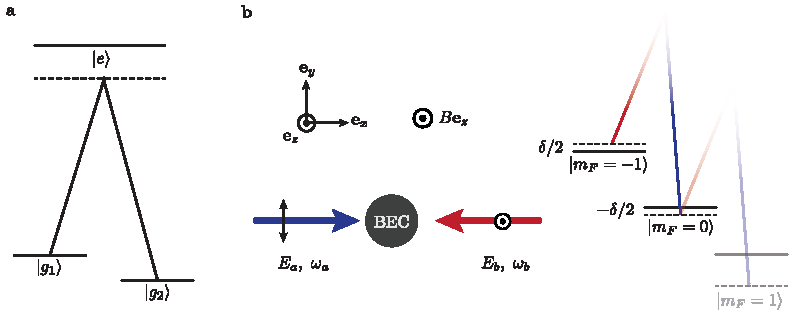
\includegraphics[]{Figures/Chapter3/Raman_coupling.pdf}
\caption[Raman coupling with two-photon transitions]{{\bf a.} A Raman transition is a two photon process that couples two ground state through and intermediate far detuned state. {\bf b.} We induce Raman transitions using a pair of cross-polarized laser beams whose and we set the difference in their angular frequencies close to the Zeeman splitting between two consecutive $m_F$ states. }
\label{fig:Raman_coupling}
\end{center}
\end{figure*}

Consider two laser beams counter-propagating along $\ex$ and with polarizations along $\ey$ and $\ez$ as is shown in Figure~\ref{fig:Raman_coupling}b. The electric field from the Raman beams is given by
%
\begin{equation}
  \mathbf{E}(x,t) = E_a\cos(k_a x-\omega_at)\e_y + E_b\cos(k_b x+\omega_bt)\ez,
\end{equation} 
%
and consequently 
%
\begin{equation}
	\mathbf{E}^*\times\mathbf{E} = 2i E_a E_b\cos(2\kl x-\omega_{a,b} t)\ex,
\end{equation}
%
where $\omega_{a.b}=\omega_a-\omega_b$. The Raman Hamiltonian is given by
%
\begin{equation}
	\hat{H}_{\rm R}=\Omega\cos(2\kl x-\omega_{a,b} t)\fx
\end{equation}
%
where $\Omega=\alpha^{(1)}g_F E_a E_b/g_J\propto \sqrt{I_a I_b}$ is the Raman coupling strength. The geometry and wavelength of the Raman fields determine the natural units of the system: the single photon recoil momentum $k_{\mathrm{L}}=2\pi/\lambda_{\mathrm{R}}$ and its associated recoil energy $E_{\mathrm{L}}=\hbar^2k_{\mathrm{L}}^2/2m$, as well as the direction of the recoil momentum $\mathbf{k}_{\mathrm{L}}=k_{\mathrm{L}}\ex$. For most experiments we tune to what is known as the `magic wavelength' or tune-out wavelength~\cite{arora_tune-out_2011} $\lambda_{\mathrm{R}}=790.034\,\nm$, at which the ground-state scalar polarizability vanishes and the scattering rate is reduced  (Figure~\ref{fig:Raman_vs_lambda}a,c). We occasionally had to tune away from the magic wavelength, for example when we were starving for laser power and wanted to increase our Raman coupling strength. An important metric for us is Raman coupling strength and Figure~\ref{fig:Raman_vs_lambda}b shows its dependence on wavelength; tuning closer to resonance allows us to decrease the laser intensity for the same experiment but comes with increased scattering rates and reduced lifetime as can be seen in Figure~\ref{fig:Raman_vs_lambda}d which shows the decay in number of Raman dressed atoms as a function of time for different wavelengths. 

\begin{figure*}[htb]
\begin{center}
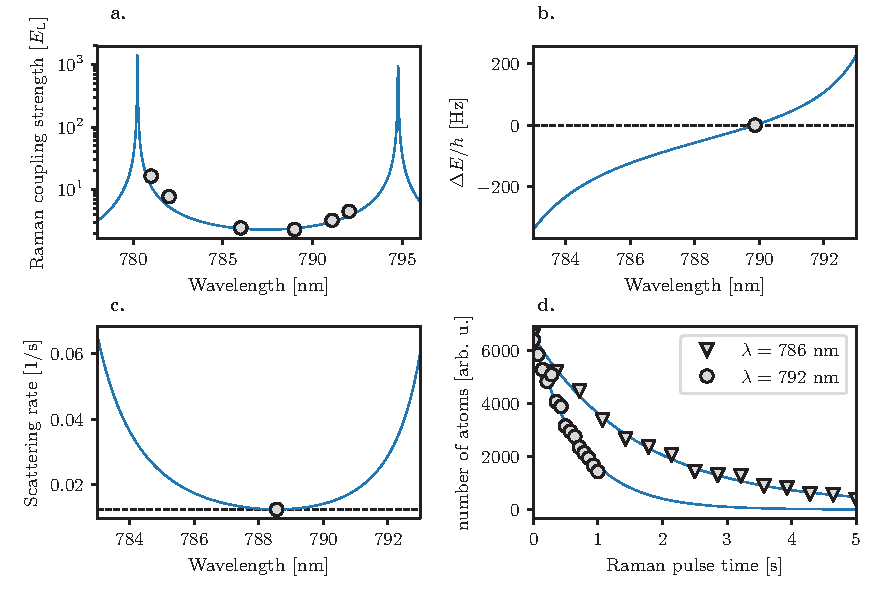
\includegraphics[]{Figures/Chapter3/electric_polarizability_anotated.pdf}
\caption[Electric realizabilities and scattering rates as a function of wavelength]{{\bf a.} Scalar polarizability as a function of wavelength near the D1 and D2 lines of $\Rb87$. We typically tune our Raman laser beams near the magic wavelength $\lambda=\unit[790.034]{nm}$. {\bf b.} Raman coupling strength as a function of wavelength measured for a pair of Raman beams with waist $w_0\sim \unit[150]{\mu m}$ and powers of $~\unit[50, 10]{mW}$. {\bf c.} Scattering rate as a function of wavelength, while it is not minimized at $\unit[790]{nm}$ its value is kept relatively low. {\bf d.} Decay in number of Raman dressed atoms as a function of hold time for the same beam parameters as in {\bf b.}. At $\lambda=\unit[786]{nm}$ the $1/e$ lifetime is $\tau=\unit[1.64]{s}$ and for $\lambda=\unit[792]{nm}$ it is reduced to $\tau=\unit[0.72]{s}$.}
\label{fig:Raman_vs_lambda}
\end{center}
\end{figure*}

In a frame rotating with angular frequency $\omega_{a,b}$ corresponding to applying the unitary transformation $\hat{U}(t)=\exp(-i\omega_{a,b} t\fz)$ and neglecting the fast terms rotating at frequency $2\omega_{a,b}$ (applying a RWA) the transformed Hamiltonian is
%
\begin{equation}
	\hat{U}^{\dagger}\hat{H}_R\hat{U} - i\hbar\hat{U}^{\dagger}\partial_t\hat{U}=\omega_{a,b} \fz+\frac{\Omega}{2}\cos(2\kl x)\fx-\frac{\Omega}{2}\sin(2\kl x)\fy,
	\label{eq:basic_Raman}
\end{equation}
%
which describes a helically precessing magnetic field with period $\lambda_{\rm R}/2$.

\subsubsection{Spin-orbit coupling}

The Raman Hamiltonian from Equation~\ref{eq:basic_Raman} can be massaged a bit more to make it look like a spin-orbit coupled (SOC)\footnote{Not to be confused with the spin-orbit coupling giving rise to the fine and hyperfine structure mentioned earlier, perhaps a better name could be spin-momentum coupling} Hamiltonian that is familiar to condensed matter physicists. If we apply a spin-dependent momentum boost which is described by the unitary operator $\hat{U}(\kl)=\exp(i2\kl x \fz)$ the full Hamiltonian including the Raman coupling and the free particle energies is transformed to
%
\begin{equation}
 	\hat{H}_{\rm{SOC}} = \frac{\hbar^2}{2m}\left(\hat q_x-2\kl\fz\right)^2+\frac{\Omega}{2}\fx + \delta\fz + \hbar\epsilon\left(\mathds{1}-\frac{\fz^2}{\hbar^2}\right),
 \end{equation} 
%
where $\delta=E_-1-\omega_{a,b}$. We can go from a 3 level system to an effective spin-$1/2$ system if we set $\Delta\omega=E_{-1}-E_0$ and consider a sizable quadratic Zeeman shift $\epsilon$, the $m_F=1$ state can be adiabatically eliminated~\cite{lin_spin-orbit-coupled_2011} and the Hamiltonian becomes
%
\begin{equation}
	\hat{H}_{SOC}=\frac{\hbar^2}{2m}(q_x-\kl\hat{\sigma}_y)^2+\frac{\hbar}{2}\Omega\hat{\sigma}_z + \frac{\hbar}{2}\delta\hat{\sigma}_y
\end{equation}
%
where $\sigma_{x,y,z}$ are the Pauli matrices. The Hamiltonian above corresponds to an equal superposition of Rashba-type~\cite{bychkov_oscillatory_1984} ($\propto \hat{\sigma}_xk_y-\hat{\sigma}_yk_x$) and Dresselhaus-type~\cite{dresselhaus_spin-orbit_1955} ($\propto -\sigma_xk_y-\sigma_y k_x$) SOC with an effective magnetic field $\propto\Omega$ in the $\ey-\ez$ plane~\cite{galitski_spin-orbit_2013,lin_spin-orbit-coupled_2011}. In Chapter~\ref{ch:Rashba} I discuss the Rashba term in more detail and introduce a way of engineering a system with only Rashba-type SOC using multiple internal levels and Raman transitions. 

\section{Detection: Resonant absorption imaging}
\label{sec:absorption imaging}

Ultracold atom experiments rely on optical imaging as the main method to probe and characterize the system. In our lab, we use resonant absorption imaging which uses a resonant probing laser that is shone at the atomic cloud and then imaged into a charged-coupled device (CCD) camera. From the absorption of the light, we can then infer properties about the atoms such as the number of atoms, temperature, integrated column density, and momentum distribution if we allow the clouds to expand. 

Consider a laser beam with intensity $I(x,y,z)$ and angular frequency $\omega$ propagating along $\ez$ through a cloud of atoms with density $n(x,y,z)$ as is shown in Figure~\ref{fig:abs_imaging_1}a. We define a (frequency-dependent) scattering cross-section $\sigma(\omega)$ which characterized the probability of an atom absorbing a probe photon and is given by the Lorentzian function
%
\begin{equation}
	\sigma(\omega)=3A_{eg}\frac{\pi^2c^2}{\omega_0^2}\frac{1}{2\pi}\frac{\Gamma}{\delta^2+\Gamma^2/4}
	\label{eq:scattering_cross_section}
\end{equation}
%
plotted in Figure~\ref{fig:abs_imaging_1}b, where $\Gamma$ is the scattering rate, $\omega_0$ is the transition frequency, $\delta=\omega-\omega_0$ is the detuning and $A_{eg}$ is the Einstein coefficient associated to spontaneous emission. As the beam travels through the cloud it will be absorbed and its intensity is reduced at a rate given by
%
\begin{equation}
	\frac{dI}{dz}(x,y,z)=-n(x,y,z)\sigma(\omega)I(x,y,z).
	\label{eq:Beer_law}
\end{equation}
%
\begin{figure*}[tb]
\begin{center}
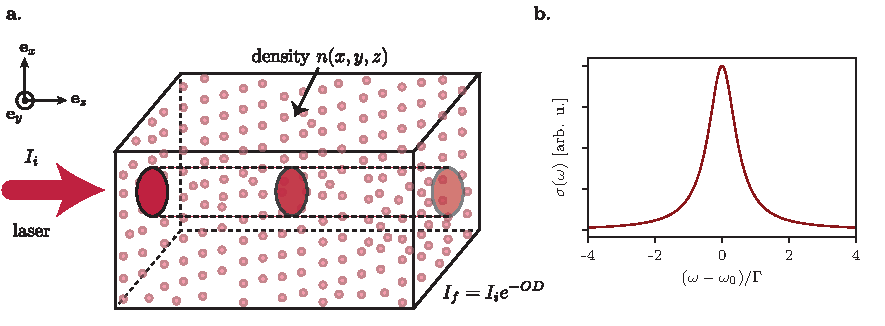
\includegraphics[]{Figures/Chapter3/abs_imaging_1.pdf}
\caption[The Beer-Lambert law]{{\bf a.} A laser beam traveling along $\ez$ through a medium with density $n(x,y,z$. The intensity decays exponentially with the integrated column density and the scattering cross section $\sigma{\omega}$. {\bf b.} The scattering cross section has a Lorentzian line shape with a full width half maximum equal to $\Gamma$. \note{TODO: add real data on panel b if I have time.}}
\label{fig:abs_imaging_1}
\end{center}
\end{figure*}

In the limit of small intensities, we can integrate this expression over the thickness of the cloud and find that the intensity decays exponentially with the density and the scattering cross section
%
\begin{equation}
	I(x,y,z)=I(x,y,0)e^{-\int_0^z n(x,y,z')\sigma(\omega)dz'},
\end{equation}

where ${\rm {OD}}=\int_0^z n(x,y,z')\sigma(\omega)dz'$ is the optical depth (OD) of the medium. If we measure the OD of the cloud it is then straightforward to obtain the integrated column density $n(x,y)$. This result, known as the Beer-Lambert law, works well when using low intensity beams. 

In the experiment we measure the optical depth of a cloud by imaging the probe into a CCD camera under two different conditions:  first in the presence of atoms to measure the attenuated intensity $I_f=I(x,y,z)$ and then without any atoms to get a measure of the initial intensity $I_i=I(x,y,0)$. The optical depth can then be computed as
%
\begin{equation}
	OD=\ln \left(\frac{I_f}{I_i}\right).
\end{equation}
%
Figure~\ref{fig:abs_imaging_2} show the different images used to compute the OD. In practice we take a third image of the background intensity $I_{\rm {bg}}$ and subtract it from the other two images.  

\begin{figure*}[htb]
\begin{center}
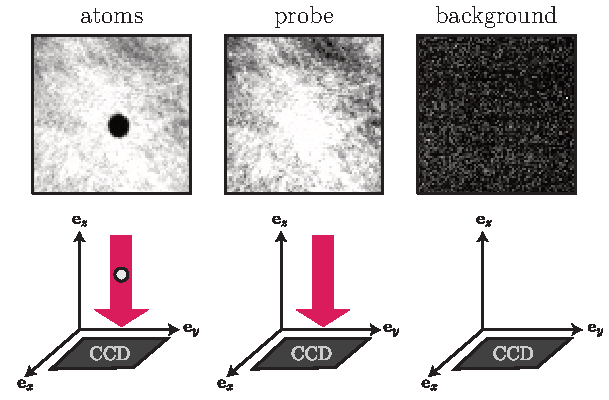
\includegraphics[]{Figures/Chapter3/abs_imaging_2.pdf}
\caption[Resonant absorption imaging]{Resonant absorption imaging. An atomic sample is illuminated with a resonant probe whose intensity is later recorded on a CCD camera. Two additional images of the unabsorbed probe intensity and the background intensity are captured in order to reconstruct the optical density of the atoms.}
\label{fig:abs_imaging_2}
\end{center}
\end{figure*}
\subsection{High intensity absorption imaging}

The use of the OD to infer the atomic density works well if we assume that the intensity of the probing laser is low such that the atoms mostly stay in the ground state. However, at high intensities a significant fraction of the atoms can become excited and effects such as stimulated emission of light have to be taken into account. As a result of this the scattering cross-section gets an additional dependence on intensity (see~\cite{Foot} for a complete derivation)
%
\begin{equation}
	\sigma(\omega, I) = \sigma(\omega)\frac{1}{{1+I/I_{\rm{sat}}}},
\end{equation}
%
where $I_{\rm{sat}}=\pi hc\Gamma/3\lambda_0^3$ is the saturation intensity, and when $I=I_{\rm{sat}}$ the population in the ground and excited state are equal. Integrating Equation~\ref{eq:Beer_law} using the modified expression for $\sigma(\omega, I)$ gives
%
\begin{equation}
	n(x,y)\sigma(\omega)=-\alpha^{\star}\ln(I_f/I_i) + \frac{I_i-I_f}{I_{\rm{sat}}},
	\label{eq:corrected_beer_law}
\end{equation}
%
where I have also added an additional dimensionless parameter $\alpha^{\star}$ which can account for imperfections in the imaging process (see~\cite{reinaudi_strong_2007}).

\begin{figure*}[htb]
\begin{center}
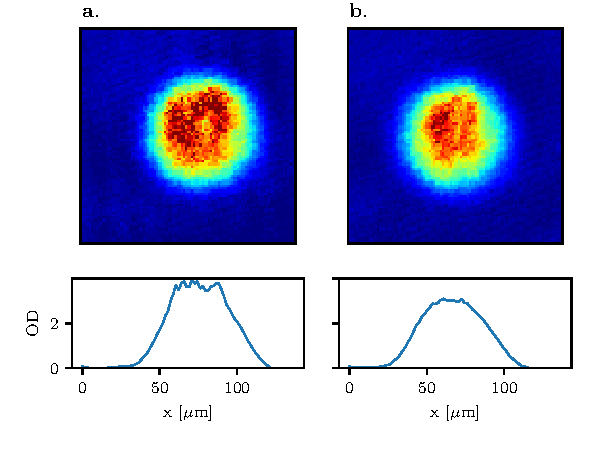
\includegraphics[]{Figures/Chapter3/flat_top_BEC.pdf}
\caption[High intensity absorption image]{{\bf a.} A BEC imaged at low intensity shows a `flat-top' density profile. {\bf b.} In order to recover the Thomas-Fermi profile it is necessary to image high density BECs with intensities larger than $I_{\rm{sat}}.$}
\label{fig:flat_top_BEC}
\end{center}
\end{figure*}

It is hard to reliably measure atomic clouds at low intensity when the OD is of the order of 3 or 4 (such as our BECs) and a significant fraction of the imaging light is absorbed. Due to the limited dynamic range of CCD cameras, the measured OD saturates resulting, for example, in imaging `flat-top' BECs rather than the usual Thomas-Fermi distribution as shown in Figure~\ref{fig:flat_top_BEC}. To get around this issue we typically image with using intensities $I>I_{\rm{sat}}$. In order to correctly compute the column density including saturation effects we need a conversion of $I_{\rm{sat}}$ from mW/cm$^2$ to counts per pixel on the CCD camera. We follow the procedure described in~\cite{reinaudi_strong_2007} find the values of $\alpha^{\star}$ and $I_{\rm{sat}}$ in counts per pixel. To learn about other effects such as the recoil momentum from the imaging light that could affect absorption images see~\cite{genkina_feshbach_2015}. 

\section{Coherent manipulation}
\label{sec:quantum_coherent_dynamics}

In this section, I describe quantum coherent processes that are driven within the electronic grounds state using the magnetic and electric dipole interactions described in previous sections. We rely on these techniques both for state preparation and characterization of our system. In all of the cases I consider a system described by the Hamiltonian 
%
\begin{equation}
	\hat{H}=\hat{H}_0+\hat{H}_I(t)
\end{equation}
%
where $\hat H_0$ describes unperturbed atomic levels and $\hat H_I(t)$ is a time dependent interaction. For simplicity I consider only a two-level system 
%
\begin{equation}
	\hat{H}_0=\hbar\begin{pmatrix}
\omega_g & 0  \\
0 & \omega_e   \\
\end{pmatrix}
\end{equation}
%
where with $\ket{g}$ and $\ket{e}$ are the unperturbed ground and excited states with energy $\hbar\omega_i$ are the energies of the unperturbed states. %Some of this techniques are generalized to three levels in Chapter~\ref{ch:Rashba}. 

\subsection{Rabi oscillations}

First I consider an interaction term that oscillates with frequency $\omega$ close to the transition energy $\omega_{ge}=\omega_g-\omega_e$ 
%
\begin{equation}
	\hat{H}_I=\hbar\begin{pmatrix}
0 & \Omega\cos(\omega t)  \\
\Omega^*\cos(\omega t) & 0   \\
\end{pmatrix}
\end{equation}
%
the coupling strength $\Omega$ here could be related to an electric dipole transition $\Omega\propto\bra{g}\mathbf{d}\cdot\mathbf{E}\ket{e}$\footnote{For our system intensities $\Gamma\gg\Omega$ and we don't observe Rab oscillations from (single photon) electric dipole transitions.} or magnetic dipole $\Omega\propto \bra{g}\boldsymbol{\mu}\cdot\mathbf{B}\ket{e}$ transition matrix element. The state of the system at any given time is given by
%
\begin{equation}
  \ket{\Psi}=c_g(t)e^{-i\omega_gt}\ket{g} + c_e(t)e^{-i\omega_e t}\ket{e},
  \label{eq:simple_Rabi}	
\end{equation}
%
and substituting this expression into the time dependent Schr\"odinger equation we find that
%
\begin{align}
	\dot{c}_g(t)=&\frac{\Omega}{2}\left(e^{i(\omega-\omega_{ge})t}+e^{-i(\omega+\omega_{ge}) t}\right)c_e \nonumber \\
	\dot{c}_e(t)=&\frac{\Omega^*}{2}\left(e^{i(\omega-\omega_{ge})t}+e^{-i(\omega+\omega_{ge}) t}\right)c_g.
\end{align}
%
We can apply a RWA if the term $\omega+\omega_{ge}$ is large compared to $\omega-\omega_{ge}$. The resulting coupled differential equations can be solved in a standard way by differentiating $\dot c_e$ one more time and substituting $\dot c_g$. If we assume that at $t=0$ the system is prepared in $\ket{g}$ the population in $\ket{e}$ describes what is known as a Rabi oscillation~\cite{rabi_space_1937}
%
\begin{equation}
	\vert c_e(t)\vert^2=\frac{\Omega^2}{\Omega^2+\delta^2}\sin^2\left(\frac{\sqrt{\Omega^2+\delta^2}}{2}t\right)
	\label{eq:Rabi_oscillations}	
\end{equation}
%
where $\delta=\omega-\omega_{ge}$ is a detuning and $\tilde{\Omega}=\sqrt{\Omega^2+\delta^2}$ is known as the generalized Rabi frequency. 
%
\begin{figure*}[htb]
\begin{center}
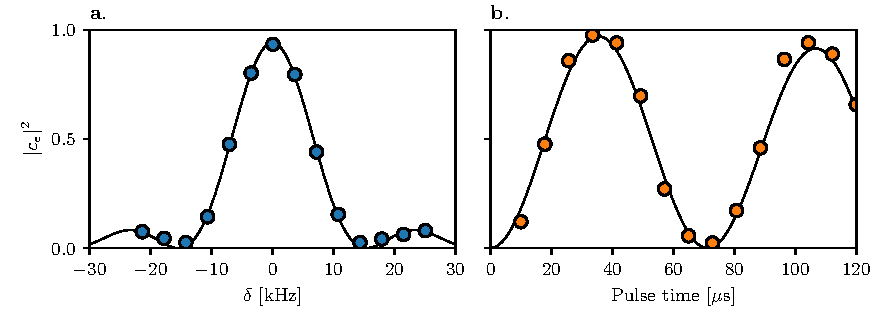
\includegraphics[]{Figures/Chapter3/rabi_cycle.pdf}
\caption[The Rabi cycle]{The Rabi cycle. Population transfered from $\ket{F=1, m_F=-1}$ into $\ket{F=1, m_F=0}$ using an RF magnetic field with $\Omega=\unit[7.1]{kHz}$. The markers indicate experimental data points and the lines correspond to fits to the model in Equation~\ref{eq:Rabi_oscillations}{\bf a.} Population transfered for a $\unit[60]{\mu s}$ pulse as a function of detuning $\delta$. {\bf b.} Population transfered as a function of time close to resonance.}
\label{fig:rabi_cycle}
\end{center}
\end{figure*}
%
The Hamiltonian after applying the RWA can be written as
%
\begin{equation}
\hat{H}_0=\hbar\begin{pmatrix}
-\delta/2 & \Omega/2  \\
\Omega^*/2 & \delta/2  
\label{eq:h_rwa}
\end{pmatrix},
\end{equation}
%
and its eigenenergies correspond to $E_{\pm}=\pm{\tilde{\Omega}/2}$. Notice that the difference between the eigenenergies $E_+-E_-$is exactly equal to the frequency at which the populations in $\ket{g,e}$ oscillate, this will come up again in Chapter~\ref{ch:Fourier_spectroscopy}. Figure~\ref{fig:rabi_cycle} shows an example of this process where we coupled an initial state $\ket{g}=\ket{F=1,m_F=-1}$ to $\ket{e}=\ket{F=1,m_F=0}$ using a radio-frequency (RF) magnetic field with $\Omega=\unit[7.1]{kHz}$. Figure~\ref{fig:rabi_cycle}a shows the population in $\ket{e}$ as a function of $\delta$ for a $\pi$ pulse ($\delta=0$, $\Omega t =\pi$). The location of the peak in this curve is as a way to find the transition frequency (we use this method in Chapter~\ref{ch:clock_states}). Figure~\ref{fig:rabi_cycle}b shows the population transfered into $m_F=0$ from $m_F=-1$ as a function of time; we typically look at the frequency of these Rabi oscillations to calibrate the coupling strength of an effective two-level system.

\subsection{Adiabatic rapid passage}
\label{sec:arp}

The Hamiltonian in Equation~\ref{eq:h_rwa} can in principle be used to transfer all the population from the initial state $\ket{g}$ into $\ket{e}$ if we set the detuning of our oscillating field to $\delta=0$ and pulse it for a time $\tau$ such that $\Omega\tau=\pi$. Unfortunately in the lab we are susceptible to noise in both $\delta$ and $\Omega$ and pulsing is not the most reliable technique for state preparation. To transfer atoms within different $\ket{F,m_F}$ states within the $5^2S_{1/2}$ hyperfine manifold we use instead an adiabatic rapid\footnote{The term rapid is with respect to the spontaneous emission rate of the excited state being coupled.} passage (ARP) protocol which is based on the Landau-Zener model~\cite{zener_non-adiabatic_1932}. 

ARP relies on preparing dressed states; eigenstates of the atomic Hamiltonian (Equation~\ref{eq:h_rwa}) which I label using the symbols $\ket{\pm}$ and dynamically changing the detuning $\delta=\delta(t)$. We start at a large and negative detuning $\delta\ll-\Omega$ where the ground eigenstate $\ket{-}\approx\ket{g}$ and therefore by slowly turning $\Omega$ on we can adiabatically prepare $\ket{-}$. We consider $\partial_t\delta>0$ so that the detuning increases with time. As $\delta$ is varied, the state decomposition of $\ket{\pm}$ changes and when $\delta=0$ they become equal superpositions of the bare states 
%
\begin{equation}
	\ket{\pm}=\frac{1}{2}\left(\ket{g}\pm\ket{e}\right).
\end{equation}
%
Finally, when $\delta\gg\Omega$ we have $\ket{-}\approx\ket{e}$ and if the change in detuning is slow enough that the system can adiabatically follow the ground eigenstate $\ket{-}$ then at the end of this process the state can be successfully transfered from $\ket{g}$ into $\ket{e}$. It can be shown that the fraction that does not adiabatically follow the ground state is given by the Landau-Zenner tunnel probability~\cite{SteckTextbook}
%
\begin{equation}
	P_{\rm{lost}}=\exp\left(-\frac{\pi\Omega^2}{2\vert\partial_t\delta\vert}\right)
\end{equation}
and in the limit of large coupling strength compared to the detuning sweep rate ($\Omega\gg\vert\partial_t\delta\vert$) all the population adiabatically follows the ground state.

In the lab we mostly use ARP with RF magnetic fields to transfer between different $m_F$ states within the $F=1$ manifold. We set the frequency of the field $\omega_{\rm{RF}}$ so that it matches the Zeeman splitting between the $m_F=-1$ and $m_F=0$ states for a target bias field $B_0\ez$. We start with atoms in $m_F=-1$ and at a bias field $B_i\approx B_0-\unit[380]{mG}$ ($\delta\approx\unit[-30]{kHz}$). We ramp an $\Omega=\unit[20]{kHz}$ RF field with angular frequency $\omega_{\rm{RF}}$ in $\unit[50]{ms}$. We then sweep the detuning by linearly changing the bias field in $\unit[50]{ms}$. Finally, the RF field is abruptly turned off, projecting the RF eigenstates back into the $m_F$ basis. In Figure~\ref{sec:arp} we set $\omega_{\rm{RF}}=\unit[23]{MHz}$ and when the Zeeman splitting between $m_F=-1$ and $m_F=0$ is equal to $\omega_{\rm{RF}}$ we observe an equal superposition of both states and if the detuning is swept beyond resonance we can reliably prepare the $m_F=0$ state. 

In general it is necessary to look at the eigenstates of the three-level RF Hamiltonian
%
\begin{equation}
\hat{H}_{\rm{RF}}=\begin{pmatrix}
-\delta & \Omega_{\rm{RF}}/2 & 0  \\
\Omega_{\rm{RF}}/2 & -\epsilon & \Omega_{\rm{RF}}/2  \\
0 & \Omega_{\rm{RF}}/2 & \delta  
\end{pmatrix},
\end{equation}
%
but for large quadratic Zeeman shifts as is usually the case in our experiments we can only look at an effective two-level system.

\begin{figure*}[!thb]
\begin{center}
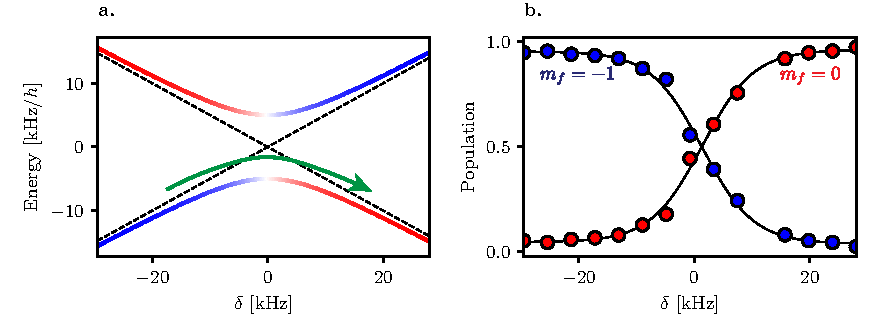
\includegraphics[]{Figures/Chapter3/arp_anotated.pdf}
\caption[Adiabatic rapid passage]{{\bf a.} Eigenenergies and eigenstate decomposition of an RF dressed Hamiltonian for a two-level system (Equation~\ref{eq:h_rwa}) with $\Omega=10$as a function of detuning. The eigenstates are linear combinations of $m_F=-1$ and $m_F=0$ (red and blue respectively). {\bf b.} Population in the $m_F$ sates for different values of detuning}
\label{fig:arp}
\end{center}
\end{figure*}

\subsection{Magnetic field stabilization with microwave assisted partial transfer absorption imaging}
\label{sec:ptai}

Most experiments in the lab are performed in the $F=1$ ground hyperfine manifold with some bias field $B_0\ez$ that shifts the energies of the different $\ket{m_F}$ states. Due to the linear dependence of the energies of the $\ket{m_F=\pm1}$ and the constant changes in the ambient magnetic field we use microwave assisted partial transfer absorption imaging (PTAI) to monitor and stabilize the magnetic field. 

The method relies on transferring a small fraction of atoms into the $5^2S_{1/2}$ $F=2$ manifold using a magnetic field with frequency close to the $\unit[6.8]{GHz}$ ground hyperfine splitting. The atoms in $F=2$ can be imaged without the use of repump light and therefore minimally disturbing the remaining atoms in $F=1$. We apply two microwave pulses for a total time $\tau$ with frequency $\omega_0-\delta_{\pm}$ where $\delta_{\pm}=\pm1/(2\tau)$. We typically set $\omega_0$ equal to the Zeeman splitting between the $\ket{F=1, m_f=-1}$ and $\ket{F=2, m_f=-2}$ states and we set the coupling strength $\Omega_0\ll 1/\tau$ such that only about $5\%$ of the atoms are transferred by each pulse. We image the transferred atoms following each pulse using absorption imaging and from the measured densities we calculate the imbalance
%
\begin{equation}
 	n_{\rm{imb}}=\frac{n(\delta_+)-n(\delta_-)}{n(\delta_+)+n(\delta_-)}
 \end{equation} 
%
\begin{figure*}[htb]
\begin{center}
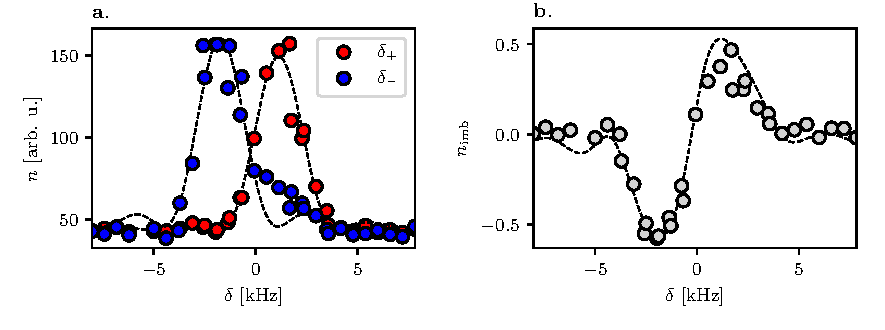
\includegraphics[]{Figures/Chapter4/uwave_lock.pdf}
\caption[Magnetic field stabilization using microwave assisted PTAI]{Magnetic field stabilization using microwave assisted PTAI. {\bf a.} Population transfered into $\ket{F=2, m_F=-1}$ from $\ket{F=1, m_F=-1}$ as a function of bias magnetic field (global detuning $\delta$). Each microwave pulse was $\tau=\unit[250]{\mu s}$ and detuned by $\delta_{\pm}=\pm 1/(2\tau)$ transfer a small fraction of atoms from $\ket{F=1, m_F=-1}$ into $\ket{F=2, m_F=-1}$. {\bf b.} Error signal calculated using the transfered atoms by each pulse. We lock the magnetic field to the $\sim\unit[5]{kHz}$ ($\unit[\sim 7]{mG}$) wide linear portion of the signal.}
\label{fig:uwave_lock}
\end{center}
\end{figure*}
which gives us a signal that is both insensitive to fluctuations in the number of atoms and linearly sensitive to changes in magnetic field\footnote{A single pulse on resonance is quadratically sensitive to detuning (see Equation~\ref{eq:Rabi_oscillations})}. We use this error signal both to monitor the magnetic field before performing experiments and cancel long term drifts in the field. In most cases, we chose the states $\ket{F=1, m_F=-1}$ and $\ket{F=2, mf=-2}$ as their relative energies are the most sensitive to changes in magnetic field. Figure~\ref{fig:uwave_lock}a shows the transfered atoms by each microwave pulse for different values of bias magnetic field and Figure~\ref{fig:uwave_lock}b shows the imbalance. The microwave frequency $\omega_0$ is on resonance with the $\ket{F=1, m_F=-1}\rightarrow\ket{F=2, m_F=-2}$ transition when both pulses transfer the same number of atoms.


In~\cite{seroka_repeated_2019} we studied partial transfer absorption imaging as a minimally destructive technique for imaging ultracold atoms. See Chapter~\ref{ch:clock_states} for an alternative solution for dealing with magnetic field noise. 

\subsection{Ramsey interferometer}
\label{sec:Ramsey_interferometer}

Now I consider a Ramsey interferometer~\cite{ramsey_molecular_1950},  a setup that is relevant to Chapters~\ref{ch:clock_states} and~\ref{ch:Rashba}. The interaction Hamiltonian is the same as in the previous section but rather than being on continuously it is pulsed on for a time $\tau=\pi/2\Omega$ (a $\pi/2$ pulse), then the system is let to evolve only under $\hat{H}_0$ for a variable time $t_{\rm{dark}}$ and finally a second $\pi/2$ pulse is applied. Figure~\ref{fig:simple_Ramsey}a illustrates this protocol: the $\pi/2$ pulses can be thought of as $\pi/2$ rotations on the Bloch sphere along $\ex$ transforming the initial state $\ket{g}\rightarrow(\ket{g}+\ket{e})/\sqrt{2}$. For the duration of the dark time, the system precesses on the equator of the Bloch sphere by an angle $\delta t_{\rm{dark}}$ and finally the second pulse rotates the state along the $\ex$ axis again. The probability of measuring the excited state is related to the phase accumulated during the dark time is given by
\begin{equation}
	\vert c_{e}(2\tau + t_{\rm{dark}})\vert^2=\left\vert \frac{\Omega \tau}{2}\right\vert\left[ \frac{\sin(\delta\tau/2)}{\delta\tau/2} \right]^2 \cos^2\left(\frac{\delta t_{\rm{dark}}}{2}\right),
\end{equation}
%   
where the oscillation frequency is only determined by the detuning. In contrast, for a Rabi oscillation the detuning adds in quadrature with $\Omega$, which suppresses the effect of the detuning when it is large as $\tilde{\Omega}\approx\Omega+\delta^2/2\Omega$. This will be important in Chapter~\ref{ch:clock_states} and additionally in Chapter~\ref{ch:Rashba} I rely on a variation of the Ramsey interferometer to perform quantum state tomography. Figure~\ref{fig:simple_Ramsey}b shows an example of a Ramsey fringe as a function of detuning $\delta$ that we measured using two states coupled with $\Omega=\unit[1]{kHz}$. 

\begin{figure*}[htb]
\begin{center}
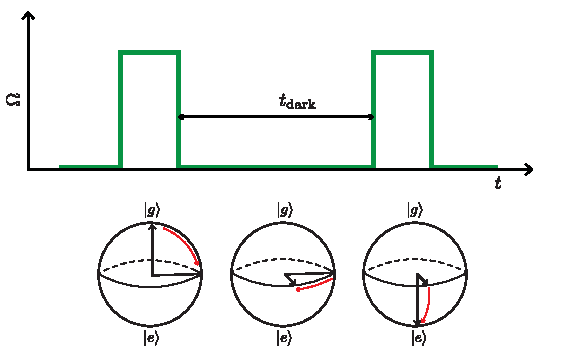
\includegraphics[]{Figures/Chapter3/Ramsey.pdf}
\caption[A Ramsey interferometer]{{\bf a.} A Ramsey interferometer: Two $\pi/2$ pulses are separated by a time $t_{\rm{dark}}$. The phase accumulated in the interferometer is equal to the detuning multiplied by the dark time. {\bf b.} A Ramsey interference fringe obtained from coupling two levels using an RF field with $\Omega=\unit[1]{kHz}$. We applied a pair of $\tau=\unit[25]{\mu s}$ pulses separated by a $\unit[50]{\mu s}$ wait and varied the detuning by changing the bias magnetic field.}
\label{fig:simple_Ramsey}
\end{center}
\end{figure*}

\subsection{Floquet theory}
\label{sec:Floquet_theory}
The RWA has been used multiple times throughout this Chapter so that the Hamiltonian describing a driven system can effectively be viewed as time-independent. This approximation is valid most of the time for our experiments, however, if we want to give a complete description of a time periodic system Floquet theory can be helpful. I will give a brief overview of Floquet theory using a matrix approach that is particularly useful for numerical computations. 

Consider a time periodic Hamiltonian $\hat{H}(t)=\hat{H}(t+T)$. We can write in terms of its Fourier components
%
\begin{equation}
	\hat{H}(t)=\sum_{j=-\infty}^{\infty}\exp[ij\omega t]\hat{H}_j,
\end{equation}
%
where $\omega=2\pi/T$ and because $\hat{H}$ is Hermitian the operators must satisfy $\hat{H}_j=\hat{H}^{\dagger}_{-j}$. The eigenstates of the Hamiltonian can be written in a terms of quasi periodic functions\footnote{Very much like Bloch wave functions}
%
\begin{equation}
\ket{\psi_{\epsilon}(t)}=\exp(-i\epsilon t/\hbar)\sum_{k=-\infty}^{\infty}\exp[-ik\omega t]\ket{\psi_{\epsilon,k}}	
\end{equation}
%
where the term $\epsilon$ is known as the quasi-energy. Inserting this expression into the time-dependent Schr\"odinger equation gives
%
\begin{equation}
	\sum_k(\epsilon+\hbar\omega k)\exp[-k\omega t]\ket{\psi_{\epsilon,k}}	=\sum_{j,j'}\exp[i(j-j')\omega t]\hat{H}_{j'}\ket{\psi_{\epsilon,j}}.
\end{equation}
In order for the equality to be true we must have $j'-j=-k$ because the complex exponentials form an orthonorormal basis and we can write
%
\begin{equation}
	\epsilon\ket{\psi_{\epsilon,k}}=\sum_j\left(\hat{H}_{j-l}-\hbar\omega k\delta_{j,k}\times\hat{\mathds{1}}\right),
\end{equation}
%
where $\hat{\mathds{1}}$ is the identity matrix. The expression can be recast into a matrix form

\begin{equation}
\epsilon\begin{pmatrix}
\cdots  \\
  \ket{\psi_{\epsilon,-1}}\\
  \ket{\psi_{\epsilon,0}}\\
  \ket{\psi_{\epsilon,1}}\\
  \cdots
\end{pmatrix}=
\begin{pmatrix}
 \hat{H}_0+2\hbar\omega  & \hat{H}_1 & \hat{H}_2 & \cdots & \cdots \\
  \hat{H}_-1  & \hat{H}_0+\hbar\omega & \hat{H}_1 & \hat{H}_2 & \cdots \\
  \hat{H}_-2  & \hat{H}_{-1} & \hat{H}_0 & \hat{H}_1  & \cdots\\
  \cdots  & \hat{H}_{-2} & \hat{H}_{-1} & \hat{H}_0-\hbar\omega & \hat{H}_1\\
  \cdots  & \cdots & \hat{H}_{-2} & \hat{H}_{-1} & \hat{H}_0-2\hbar\omega \\.
\end{pmatrix}
\end{equation}

The quasienergies $\epsilon$ can be computed by truncating and then diagonalizing the matrix, and they are grouped into repeating manifolds separated in energy by $\hbar\omega$. The quasienergies within a manifold can be interpreted as the eigenenergies of an effective time-independent Hamiltonian $\hat{H}_{Fl}$ that describes the evolution of the system sampled stroboscopically at an integer number of driving periods, with the time evolution operator $\hat{U}(t_0,t_0+T)=e^{-iT\hat{H}_{Fl}}$. 

Floquet theory played an important role in the engineering of different dispersion relations for atoms in Chapters~\ref{ch:Fourier_spectroscopy} and \ref{ch:Rashba}. I will give an example based on \cite{campbell_magnetic_2016}, where we considered a pair of Raman beams driving transitions between the $m_F$ states with two different frequencies $\omega_{-1,0}$ and $\omega_{0,+1}$ set to the $m_F=-1\rightarrow m_F=0$ and $m_F=0\rightarrow m_F=1$ transitions. By performing independent RWAs with respect to each of these transitions we found that the system could be described by a magnetic Hamiltonian
%
\begin{equation}
 \hat{H}=\frac{\hbar k^2}{2m}+\boldsymbol{\Omega}(x)\cdot\hat{\mathbf F} + \Omega_2 \hat F_{zz}^{(2)} 	
 \label{eq:spin_one_soc}
 \end{equation}  
%
with $\boldsymbol{\Omega}_1(x)/\Omega_1=\cos(2\kr x)\ex-\sin(2\kr x)\ey$,  $\hat F_{zz}^{(2)}\hbar=\fz^2/\hbar^2-2/3$ is an element of the quadrupole tensor and $\Omega_2=(\omega_{-1,0}-\omega_{0,1})/2$ can be interpreted as an effective quadratic Zeeman shift. The competing contributions between kinetic and magnetic ordering energies gave rise to different magnetic phases. Figure~\ref{fig:spin_one_soc}a. shows the ground branch of the dispersion relation for small $\Omega_1<4\El$ (top) and large $\Omega_1>4\El$ (bottom). As the value of $\Omega_2$ is decreased the magnetization in the system changes as the location of the global minima in the dispersion changes. The experimental parameters $\Omega_1$ and $\Omega_2$ spanned a two-dimensional phase diagram shown in Figure~\ref{eq:spin_one_soc}b that we experimentally mapped. The eigenenergies of Equation~\ref{fig:spin_one_soc} are plotted in Figure~\ref{fig:spin_one_soc}c. However in order to get a good agreement between the experiment and the phase diagram we had use the full Floquet Hamiltonian which results in having modified parameters in Equation~\ref{eq:spin_one_soc} $\Omega_2^{(\rm{eff})}= \Omega_2 + \mathcal{O}(\Omega_1^2/\epsilon)$ (red dotted line in Figure~\ref{fig:spin_one_soc}b). Figure~\ref{fig:spin_one_soc}d shows three manifolds of Floquet quasienergies for this system, illustrating their periodic nature.

\begin{figure*}[!htb]
\begin{center}
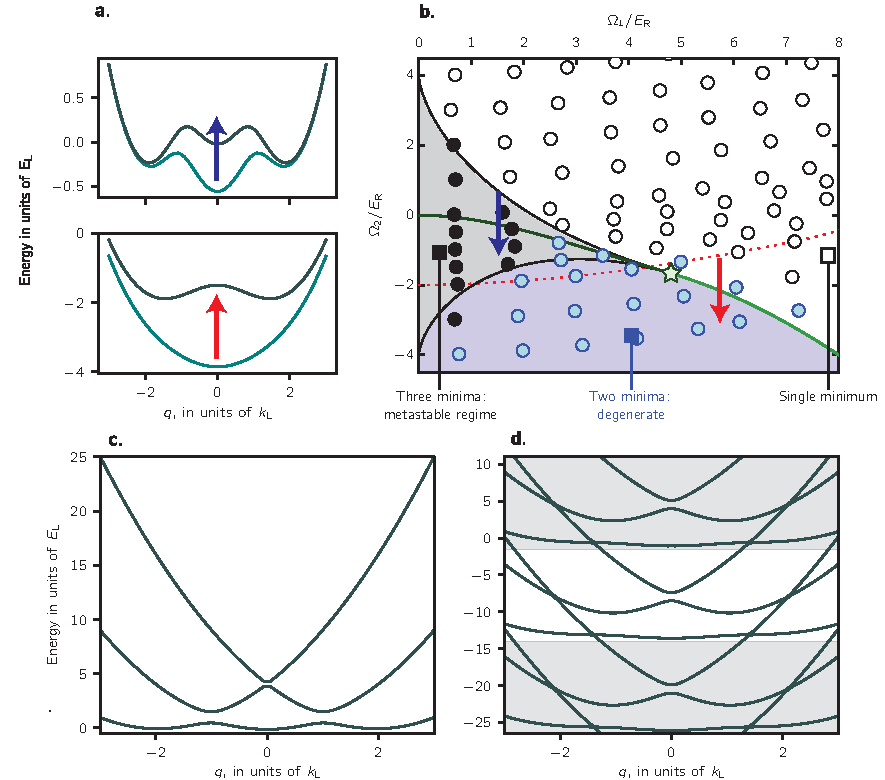
\includegraphics[width=\textwidth]{Figures/Chapter3/spin_one_floquet.pdf}
\caption[Magnetic phases of a spin-1 SOC system]{Magnetic phases of a spin-1 SOC system. {\bf a.} Ground state energies of a spin-1 SOC system for $\Omega_1=\unit[1.5]\El$ (top) and  $\Omega_2=\unit[1.5]\El$(bottom). By changing $\Omega_2$ we moved the location of the central minima. {\bf b.} Phase diagram of a spin-1 SOC system. They green line corresponds to a line of phase transitions where the system goes from magnetized to unmagnetized. {\bf c.} Dispersion relation computed for $\Omega_1=\unit[2]\El$, $\Omega_2=0$. {\bf d.} Floquet qasienergy dispersion relation for the same parameters. The magnitude of $\Omega_1$ effectively modifies $\Omega_2$ in the RWA Hamiltonian.}
\label{fig:spin_one_soc}
\end{center}
\end{figure*}

%\note{TODO: if there is time I might add my own calibration data.}. 



%%%%%%%%%%%%%%%%%%%%%%%%%%%%%%%%%%%%%%%%%%%%%%%%%%%%%%%%%%%%%%%
%
%Graveyard
%
%%%%%%%%%%%%%%%%%%%%%%%%%%%%%%%%%%%%%%%%%%%%%%%%%%%%%%%%%%%%%

% The eigenstate of the perturbed Hamiltonian are linear combinations of the unperturbed eigenstates $\ket{n}$  
% %
% \begin{equation}
% 	\ket{\psi}=\sum_n a_n(t)e^{-iE_n t/\hbar}\ket{n},
% \end{equation}
% %
% using the time-dependent Schr\"odinger equation we can find equations for the coefficients $a_n(t)$
% %
% \begin{equation}
% 	i\hbar \partial_ta_n(t)=\sum_k\bra{n}\hat{H}_{\rm{dip}}\ket{k}a_k(t)e^{i\omega_{n,k}t}
% \end{equation}
% %
% where $\omega_{nk}=(E_n-E_k)/\hbar$. If we consider the perturbation being turned on at $t=0$ and if $\omega\neq\omega_{nk}$ the first order coefficient is
% %
% \begin{equation}
% 	a_n^{(1)}=-\frac{\bra{n}d_iE_0\ket{m}}{2\hbar}
% \end{equation}

% For $S$ electrons the hyperfine splitting can be described by the Hamiltonian $\hat H_{\rm{hfs}} = A_{\rm{hfs}}\mathbf{I}\cdot\mathbf{J}$\footnote{Notice how both the fine and hyperfine structure arise from a spin-orbit coupling interaction, we will discuss a very different type of spin-orbit coupling in future chapter.}. Figure~\ref{fig:fs_hfs}c shows the fine structure getting further split into states of total angular momentum $\mathbf{F}=\mathbf{J}+\mathbf{I}$. $\Rb87$ has a nuclear spin $I=3/2$ and therefore its ground state hyperfine configuration has $F=1$ and $F=2$. Here
% ~\cite{Steck} 

% Lets now consider the example of an atom in the presence of an oscillating electric field with amplitude $E_0$ and polarization $\epsilon$ $\mathbf{E}=E_0\cos(\omega t)\boldsymbol{\epsilon}$. We will use time-dependent perturbation theory to calculate the resulting energy shifts. 


% So far I have considered that the excited state has an infinitely long lifetime and does not decay. However, in reality the atom can spontaneously emit photons and decay. The lifetime of the excited state is given by $1/\Gamma_{e_j}$. The exponential decay of the excited state corresponds to adding a imaginary contribution to the energy $E_{e_j}\rightarrow E_{e_j}-i\hbar\Gamma_{e_j}/2$ which makes the polarizability a complex valued number. 

% The decay rate of a transition is related to the square of the dipole matrix element via Fermi's golden rule~\cite{Sakurai}

% \begin{equation}
% 	\Gamma_{J_gJ_e}=\frac{\omega_0^2}{3\pi\epsilon_0\hbar c^3}\frac{2J_g+1}{2J_e+1}\vert\langle g \| \mathbf{d}\|e\rangle\vert^2
% \end{equation}

% where $\vert\langle g \| \mathbf{d}\|e\rangle\vert^2$ is a reduced matrix element
% I will now look at the scalar polarizability term for Alkali atoms. For the case of far-detuned light such that the hyperfine $F$ levels are not well resolved the scalar polarizability can be calculated using the fine structure $J$ states. For an atom in an initial state $J$

% use scattering rate to find reduced matrix element write final expresion. skip the j, go back to generic notation
% %
% \begin{equation}
%  	\alpha^{(0)}\approx\sum_{J'}\frac{\vert\langle J \| \mathbf{d}\|J'\rangle \vert^2}{3\hbar}\left(\frac{1}{\omega+\omega_{JJ'}}-\frac{1}{\omega-\omega_{JJ'}}\right)
%  \end{equation} 
% If we consider Alkali atoms in the ground state hyperfine manifold in the presence of far detuned light such that the hyperfine levels are not well resolved we need to calculate the matrix elements using the $J$ states


% the scalar polarizability takes the form 
% The matrix element in Equation~\ref{eq:scalar_pol} can be expressed using the Wigner-Eckart theorem~\cite{Sakurai} in terms of the Clebsch-Gordan coefficients and the reduced matrix elements. 
%Here I will only consider the case of oscillating electric fields $\mathbf{E}=E_0\cos(\omega t)\boldsymbol{\epsilon}$ (i.e. plane waves of electromagnetic radiation) which are relevant to our experiments. 

% write tensor polarizability, write it into irreducible components. Mention that tensor component is very small and ignored. 

% Scalar polarizability: real part is light shift, complex part is scattering. Apply rwa and get the classic expressions for trapping potential and scattering. Make plot of polarizabily for RB87 Sub subsection: dipole traps

% Tensor polarizability



% Can break interaction into scalar, vector and tensor part. Interaction can also be resonant or off-resonant.

% \note{Why do you only get second order perturbation theory effects? I think it has something to do with unperturbed atomic states being eigenstates of the parity operator}

% We use light tuned to the magic wavelength $\lambda_{\mathrm{R}}=790.032\,\nm$ so that the scalar light shift vanishes (Section~\ref{sec:scalar_light_shift}). Because the light is considerably detuned from the D1 and D2 lines we do not take into account coupling into any of the excited states\footnote{Some atoms are inevitably excited of course, leading to heating from spontaneous emission (Equation~\ref{eq:scattering})}

% \note{Something about what we use this transitions for and how we usually ignore all other levels. (???)}

% \note{TODO: what about matrix elements between -1 and +1?. Move to intro chapter}

% A typical calibration of $I_{\rm{sat}}$ in counts per pixel consists in making a dilute cloud of atoms (for example a thermal cloud) and imaging it for a different range of probe intensities. In Figure \note{TODO: make i_sat plot} I'm plotting the uncorrected OD for a small portion in the center of a thermal cloud as a function of $I$. At small intensities the OD is constant but as $I$ becomes comparable to $I_{\rm{sat}}$ it starts decreasing. 

% This wavelength lies in between the D1 and D2 and it corresponds to when the red-detuned contribution to the polarizability from the D2 line is equal to the blue detuned contribution from the D1 line as is illustrated in Figure \note{TODO: make figure of scalar polarizability}.

% which is illustrated in Figure~\ref{fig:B_eff}. \note{Maybe get ride of this figure and use stuff from spin-1 paper directly.}

% \begin{figure*}[htb]
% \begin{center}
% 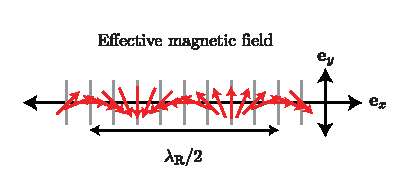
\includegraphics[]{Figures/Chapter3/B_eff.pdf}
% \caption[Effective magnetic field from two cross polarized Raman laser beams]{The effective Raman Hamiltonian can be visualized as an interaction with an effective helically precessing magnetic field.}
% \label{fig:B_eff}
% \end{center}
% \end{figure*}


% \note{TODO: the two-level stuff maybe doesn't really make much sense anymore}
